In order to understand and unreveal the properties of the charge divergences, we decided to 
extract a simple picture (and possibly equations) that reproduces the 
underlining problem. 

First, we start introducing a local effective interaction, described by RPA formula
with strong magnetic fluctuations:
\begin{equation}
	U_{\mathrm{eff},\Omega} = \int_{\bs{Q}} \frac{U}{1- U \Pi_{\bs{Q},\Omega}}.
\label{pl:ueff}
\end{equation}
Since the bare interaction $U$ is local, $U_{eff}$ depends only on the exchange 
frequency $\Omega$ from the \textit{particle-hole} bubble:
\begin{equation}
	\Pi_{\bs{Q},\Omega} = \frac{1}{\beta} \sum_{\nu} \Pi_{\bs{Q},\Omega}(\nu) 
	= \frac{1}{\beta} \sum_{\nu} \int_{\bs{p}} G_{0,\bs{p},\nu} G_{0,\bs{p}+\bs{Q},\nu+\Omega}.
\end{equation}
Where we introduced also the $\nu$-dependent bubble $\Pi_{\bs{Q},\Omega}(\nu)$, since, as we will 
see, it plays a special role in the origin of the charge divergences.

The magnetic effective interaction (\ref{pl:ueff}) will generate important effects on the other channels. 
At lowest level, for instance, we can use a ladder formula to see its role to the charge channel:
\begin{equation}
	\mathcal{C}_{\bs{Q},\Omega} (\nu,\nu') = U_{\mathrm{eff},\nu-\nu'} \left[ \delta_{\nu,\nu'} + U_{\mathrm{eff},\nu-\nu'}\Pi_{\bs{Q},\Omega}(\nu) \right]^{-1}.
\label{pl:charge}
\end{equation}
We note that, in the case of a frequency independent effective interaction $U_{\mathrm{eff}}$, Eq.(\ref{pl:charge}) becomes $\nu$ and $\nu'$ independent 
and only the summed bubble $\Pi_{\bs{Q},\Omega}$ appears, raising to an equation similar to Eq.(\ref{pl:ueff}).
Hence, the frequency dependence of the effective interaction $U_{eff}$, inside a ladder formula, changes dramatically the frequency structure of the 
resulting channel. 

\begin{figure*}
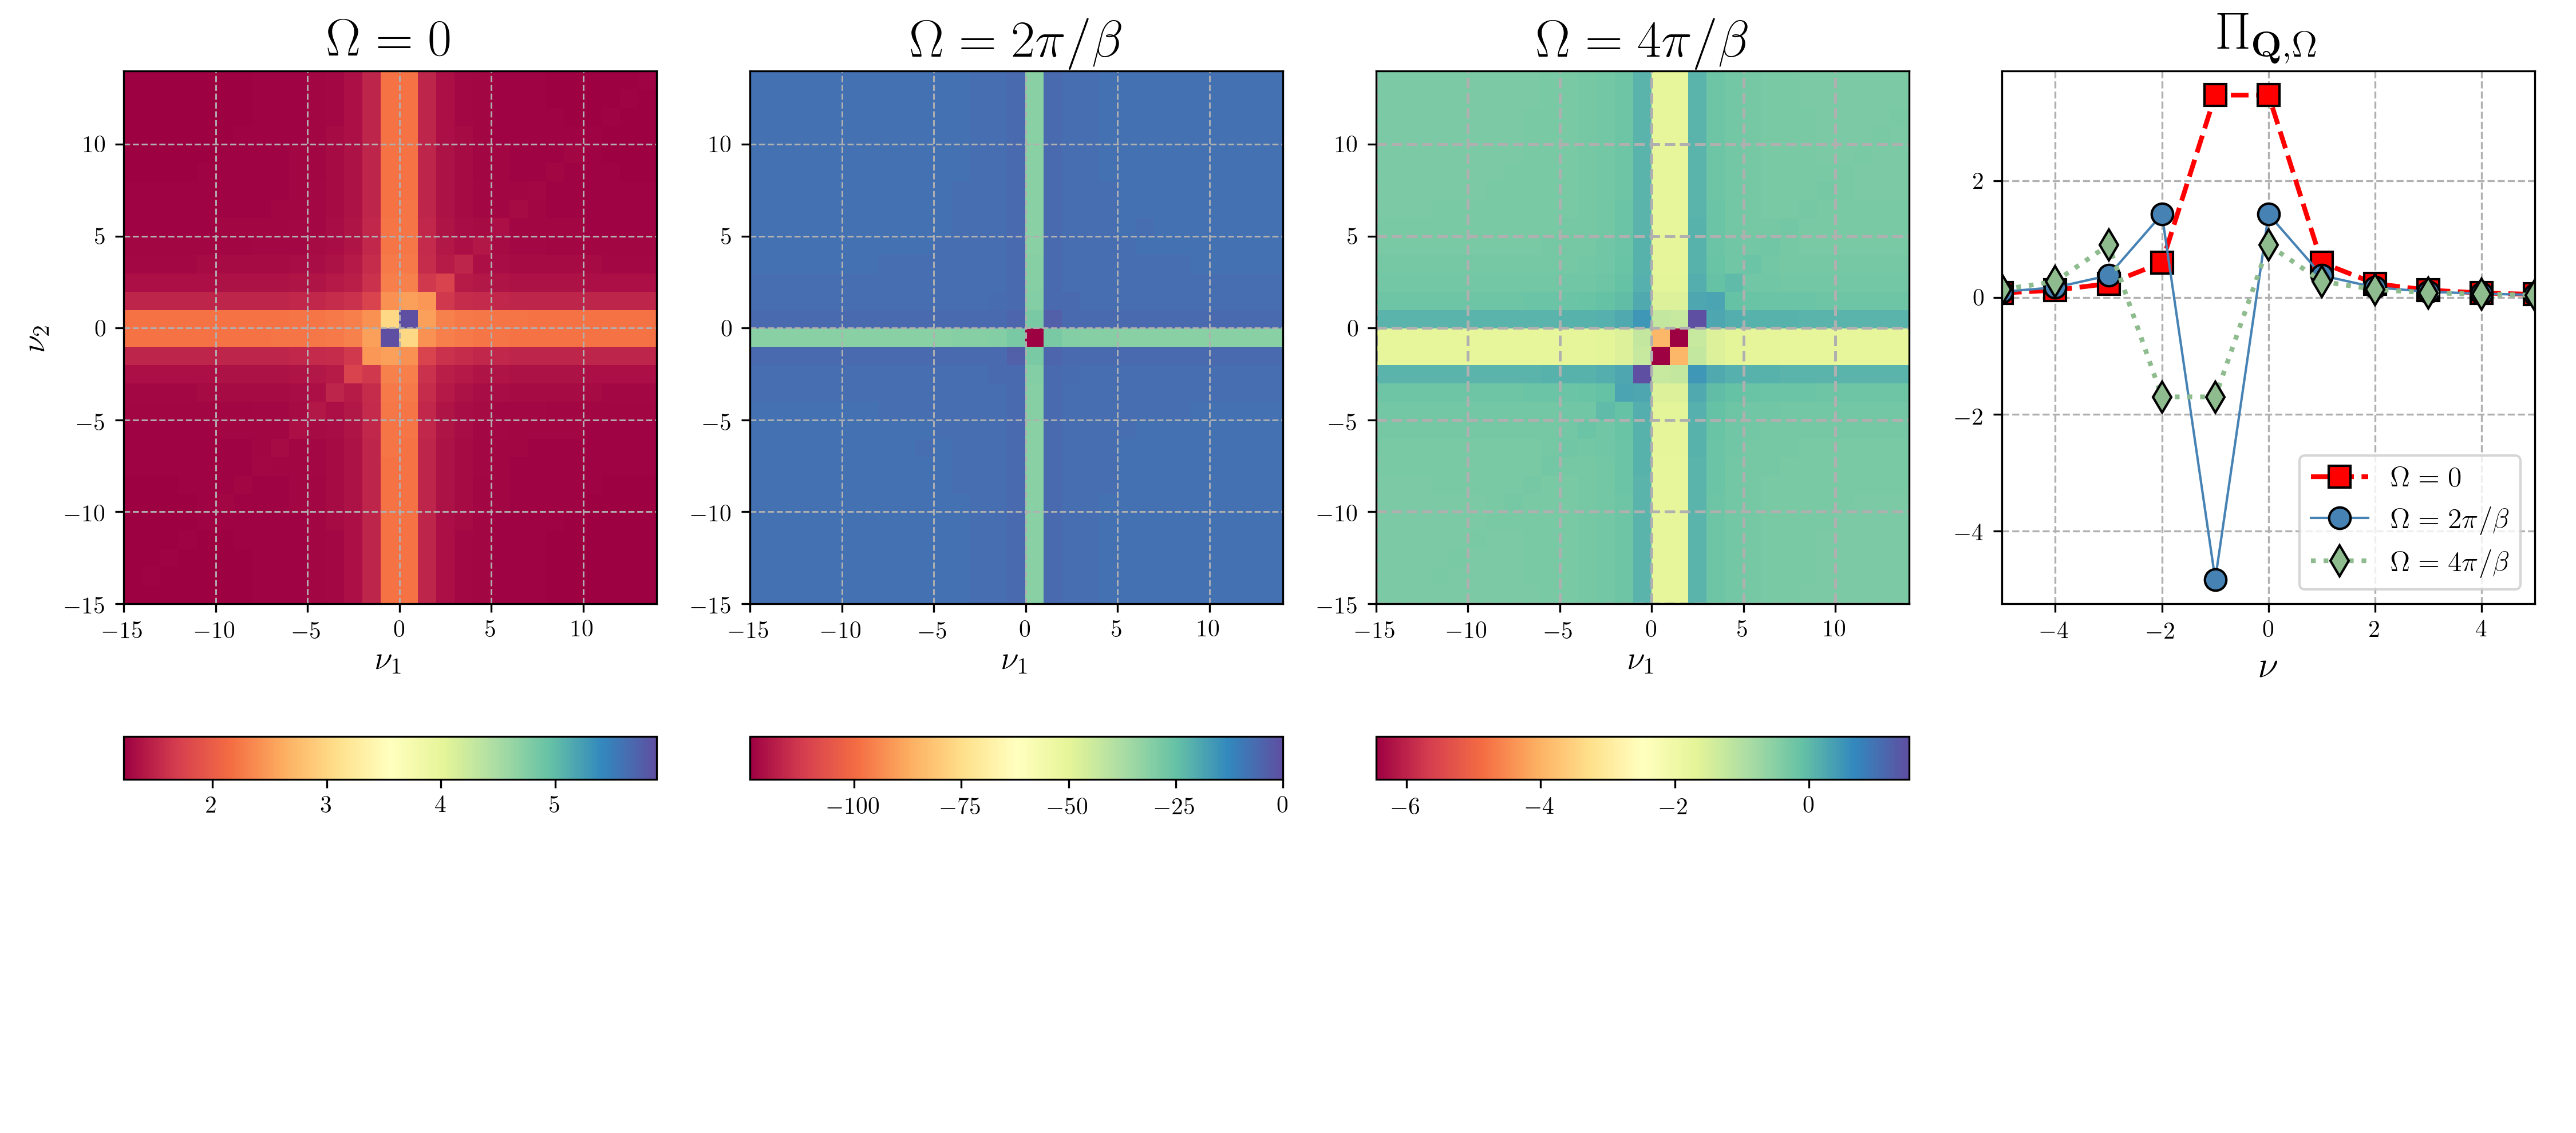
\includegraphics[width=\textwidth]{images/PL_all.png}
\vspace*{-2.0cm}
\caption{In the first three panels from the left, the charge channel $\mathcal{C}_{\bs{Q},\Omega} (\nu,\nu')$ as in Eq.~\ref{pl:charge} is shown as 
a function of $\nu$ and $\nu'$ for frequency $\Omega=0$, $\Omega=2\pi/ \beta$ and 
$\Omega=4\pi/ \beta$, respectively, for $\bs{Q}=(0,0)$. In the most right panel, the bubble $\Pi_{\bs{Q}=(0,0),\Omega}(\nu)$ is shown as a function of $\nu$ for 
$\Omega=0$, $\Omega=2\pi/ \beta$ and $\Omega=4\pi/ \beta$. All plots refer to parameters $T=1.0$, $t'=-0.32$, $x=0.375$ and $U=4$.  } 
\label{fig:perpladder}
\end{figure*}

In Fig.~\ref{fig:perpladder}, we show Eq.(\ref{pl:charge}) for different $\Omega$, $\bs{Q}=(0,0)$ and as a function of $\nu$ and $\nu'$, 
for $T=1.0$, $t'=-0.32$, $U=4$ and $x=0.375$. 
As we observe, the frequency structure for $\Omega=2\pi/ \beta$ is identical as shown in Fig.~\ref{bla}. Hence, formula (\ref{pl:charge}) 
reproduce the frequency structure of the divergence of the charge channel. The charge diverge for some finite temperature.

To understand why the divergence appears for finite frequency $\Omega$, we notice that in Eq.(\ref{pl:charge}) the $\Omega$ dependence 
appears only through the bubble $\Pi_{\bs{Q},\Omega}(\nu)$ that, as widely known, for $\bs{Q}=(0,0)$ obeys 
the following properties:
\begin{equation}
	\Pi_{\bs{Q}=(0,0),\Omega} = \frac{1}{\beta} \sum_{\nu} \Pi_{\bs{Q}=(0,0),\Omega}(\nu) = \rho_{0} \delta_{\Omega,0}.
\label{pl:sumrule}
\end{equation}
In the most right panel in Fig.~\ref{fig:perpladder}, we show the bubble $\Pi_{\bs{Q}=(0,0),\Omega}(\nu)$ as a function of $\nu$.
We note that it has a negative pick for $\Omega=2\pi/ \beta$. This is due to the property (\ref{pl:sumrule}), since the summed 
bubble must be zero for $\Omega \neq 0$ while $\Pi_{\bs{Q}=(0,0),\Omega}(\nu)$ has an analytical $\Omega$-indipendent behavior 
in the asymptotic regime $\nu \gg \Omega$.
%However, since the $\nu$ dependent bubble $\Pi_{\bs{Q}=(0,0),\Omega}(\nu)$ is non zero for any value of $\Omega$, 

